
\section{Durchführung}
\label{sec:Durchführung}
\begin{figure}[H]
  \centering
  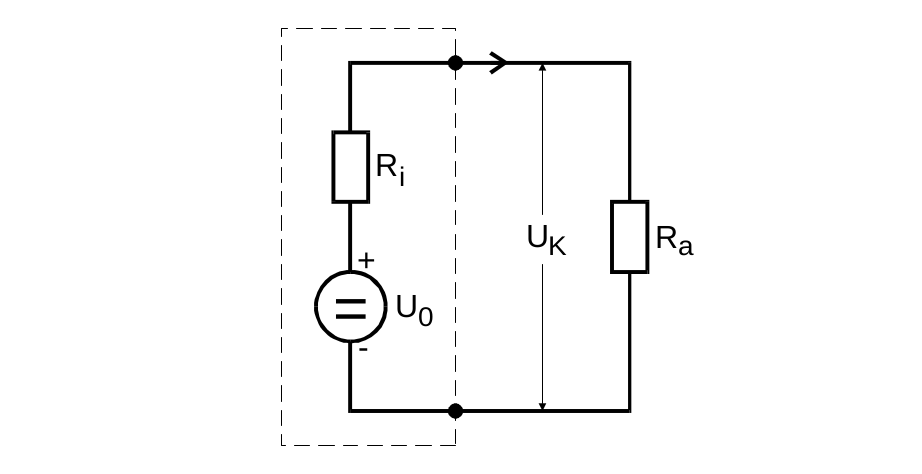
\includegraphics[width=0.9\textwidth]{Bilder/Abbildung1.png}
  \caption{Ersatzschaltbild einer Monozelle \cite{Anleitung}}
  \label{fig:abbildung1}
\end{figure}
Zur Bestimmung der Leerlaufspannung $U_0$ einer Monozelle wird diese direkt an der Monozelle wie in Abbildung \ref{fig:abbildung1} dargestellt, mit einem Spannungsmesser abgegriffen.
Zur weiteren Berechnung wird zudem der Innenwiderstand $R_V$ des Voltmeters am Messgerät abgelesen.
Im Folgenden soll nun die Klemmenspannung $U_k$ der Monozelle in Abhängigkeit vom Belastungsstrom $I$ gemessen werden.
Dazu werden, wie in Abbildung \ref{fig:abbildung2} zu sehen, ein Amperemeter und ein regelbarer Widerstand $R_a$ in Reihe geschaltet mit der Monozelle. Das Voltmeter dient nun zur Messung der Klemmenspannung $U_k$ und bleibt daher weiterhin parallel geschaltet zur Monozelle.
Der Belastungswiderstand $R_a$ wird hierbei variiert im Bereich $0-50\si{\ohm}$.
Es sollen mindestens ?=?? Wertepaare der Spannung $U_k$ in Abhängigkeit des Stroms $I$ aufgenommen werden.




\begin{figure}[h]
\centering
\begin{subfigure}{0.53\textwidth}
\centering
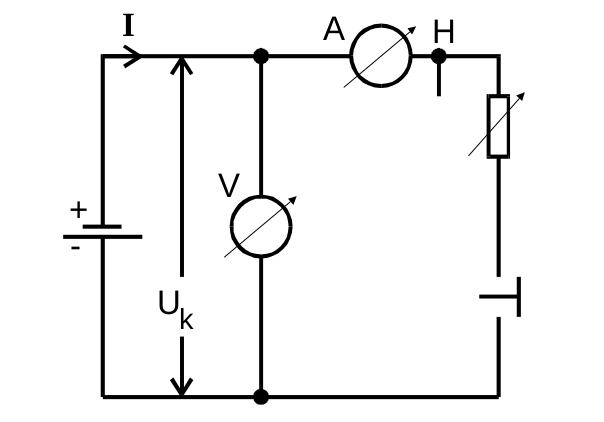
\includegraphics[width=0.9\textwidth]{Bilder/Abbildung2.png}
\caption{Messschaltung zur Bestimmung von $R_i$ und $U_0$ \cite{Anleitung}}
\label{fig:abbildung2}
\end{subfigure}
\begin{subfigure}{0.45\textwidth}
\centering
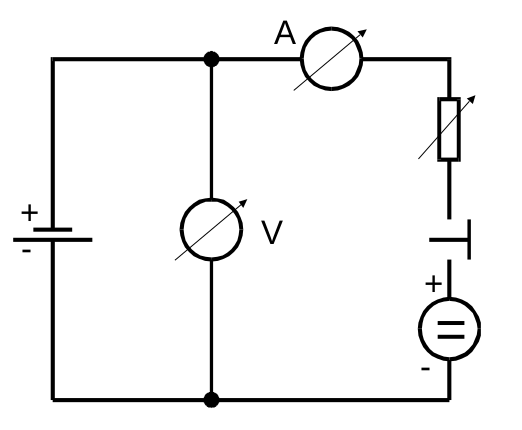
\includegraphics[width=0.9\textwidth]{Bilder/Abbildung3.png}
\caption{Messschaltung \refeq{fig:abbildung2} erweitert um eine Gegenspannung \cite{Anleitung}}
\label{fig:abbildung3}
\end{subfigure}
\end{figure}
In der nächsten Messung soll eine zusätzliche Spannungsquelle in den Schaltkreis eingebracht werden.
Diese soll hierbei $\SI{2}{\volt}$ größer sein als die Leerlaufspannung $U_0$ der Monozelle.
Die neue Spannungsquelle wird hierbei, wie in Abbildung \ref{fig:abbildung3} dargestellt, in entgegengesetzer Stromrichtung in Reihe zum Widerstand $R_a$ geschaltet.
Der Strom wird nun also in entgegengesetzter Richtung fließen. Wie bereits in der Messung zuvor wird der Widerstand erneut im Bereich $0-50\si{\ohm}$ variiert und die entsprechenden Werte der Spannung $U_k$ in Abhängigkeit des Strom $I$ notiert.

Nun wird die Monozelle aus der Schaltung ausgebaut und durch einen RC-Generator ersetzt. Wie bereits für die Monozelle soll mit der Schaltung in Abbildung \ref{fig:abbildung2} erneut die Klemmenspannung $U_k$ in Abhängigkeit zu $I$ bestimmt werden. Zunächst wird dazu der 1-V- Rechteckausgang des RC-Generators verwendet, der Widerstand $R_a$ soll hierbei variiert werden im Bereich $20-250\si{\ohm}$.
In einer weiteren Messung wird der 1-V-Sinusausgang des RC-Generators verwendet, hierbei wird $R_a$ von $0.1-5.0\si{\kilo\ohm}$ variiert.
